\section{azureml-core (Python SDK)}
% I want to be this guy, who builds with his team an increatiable A.I: system for munich.

\subsection{Connect to Workspace}
A workspace is a resource, which is tied (child) to a subscription and a resource group. A workspace links the different object to run a \gls{ML} model: Experiment, Training, Deployment. A workspace comes with a \gls{SDK} to interactive with.\\

To connect to the workspace, the constructor requires different parameters
\begin{lstlisting}[style=python]
	Workspace(
	subscription_id, resource_group, workspace_name,
	auth=None,
	_location=None,
	_disable_service_check=False,
	_workspace_id=None,
	sku='basic',tags=None, _cloud='AzureCloud'
	)
\end{lstlisting} 


\begin{comment}


There are different ways to connect to the workspace. 
\paragraph*{VSCode} allows for the use of a extension: \textit{Azure ML}. This allows to configure the connection by an \gls{IDE}. This allows also to use the \textit{compute instance} linked to the workspace as a \gls{VM}.\\

For this a kernel needs to be selected. 
%%
\paragraph{sdfsdf}
%veu
%vm
%kernel

% Python interpreter -> Python Virtual Machine
% Python interpreter & compiler
% High level language (source) code
% Binary or machine code
% Python interpreter is CPython and writen in C
% PVM converts a byte code into a bit code 
% Python interpreter Pythion 3.10 (.exe file?
% Different python version are different python programmes: This programm is called the interpreter. You can interacte with it directly over the command line (Input for the programm), which "interpretes" you high-level code and returns the output, after the interpreter is converting you high-level code into machine code.* Note: A compiler has basically the same goal, but it is doining it a bit differently.
% You could alsow provide a scipt for you interpreter, which then returns the output of this script. The IDE allows you, to better develop a python script or scripts, which then in turn is calles a python programm. A better naming, would be  a *high level programm.

% Kernel: For example. A different kernel is build, maybe for interacting with different languages (own language interpreter). The IPython with the ipykernel is build to "interprete" python and markdown/latex source code. While the IDE allows to select for different 
So each \gls{VEN} installs a kernel (ipykernel) with IPyhton (Housing). 

You alsow install jupter-lab (evolution for IPyhton) in your ven

https://www.wrighters.io/using-multiple-kernels-in-jupyter/	
C:\Anaconda3
(my_env) λ jupyter --version
Selected Jupyter core packages...
IPython          : 8.9.0
ipykernel        : 6.21.1

\begin{figure}[H]
	\centering
	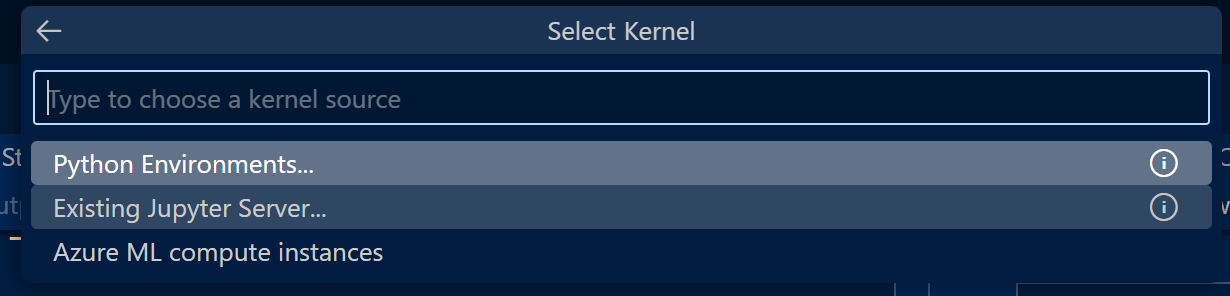
\includegraphics[scale = 0.3]{attachment/chapter_AML/Scc001}
	\caption{Connect to the workspace: Select kernel}
\end{figure}

We started, with writing the configuration file.
A started with opening jupter notebook and den selecting the kernel. And a kernel was installed on the compute cluster.
The authen

\\
auth
ServicePrincipalAuthentication or InteractiveLoginAuthentication or MsiAuthentication
default value: None
The authentication object. For more details, see https://aka.ms/aml-notebook-auth. If None, the default Azure CLI credentials will be used or the API will prompt for credentials.


\begin{lstlisting}[style=python]
	from azureml.core import Workspace
	ws = Workspace.create(name='myworkspace',
	subscription_id='<azure-subscription-id>',
	resource_group='myresourcegroup',
	create_resource_group=True,
	location='eastus2'
	)
	
	for i in range(n):
	print('i = ', i)
\end{lstlisting}


\subsection{*Kernels}
Form your local machine, you don't need to create an enviroment. You select a kernel. For this, you are not
using the local CPU to run, but you are using the compute instance. 

A bit of definition first:

Understanding a kernal an how it is connected to an environment.

Kernel: is a program that runs and introspects the user’s code.

Conda env: is a directory that contains a specific collection of conda packages that you have installed.

These 2 concepts are describing different things, kernel is like an executable, conda env is the resources (packages) at this executable’s dispose.

Selecting the compute instance, we are acturally in a visturel machine, not only a virtual enviroment. This will be 

That will be important, by selecting the compute instance, you accessing the vistural machine (which is not you local machine). Therefore the virtual envoroment will be installed over there.

For example, therefore the command write the configuration file, will create a problem. Because it seams to be, that I'm not allowed to write in the directory of the virtual machine.

Now.
the next question is, is it possible to use the internal kernal on you own machine, to excute the code.

For now, it is without the kernal form 

so the .exe in the conda enviroment is a kernal?

---- Okay, make something clean.
What I'm now testing, if i get the specific workspace configuration.
The probelm is, how do we can manage all does different access points, while having one repsository to connect to?
Questions over questions.
It is still unclear, what the difference between an interpreter and an kernel is.
For this purpose, there is no difference. it is a computional 

The \textit{IPython} with it's \textit{ipykernel} as a default kernel (as \textit{ipykernel}). 
Other language kernels are available for the jupter notebook.

IPython is XXX and ipykernel is the actually kernel. However, I still don't understand. To the question is, that 

What happen, if you select the ipykernel for in the compute instance. 
So what happens here.
The nice thing is, that I actually starting to making progress in this area.
Very, very good.

Now back. What the fuck is an interpreter, the languages it self and an kernel. The kernel think, I have the sense, it's very important, to understant. Not as a essetion question to solve it. But as a basiline knowleadge question, it seems to be nessary.

Fucking kernel.

Now, let's start anyway.

Add the pictures to

The \gls{g_Kernel} to excute the code, needs to be selected. ITE


Now, now, 

path, where the interpreter is saved?
It depends, 
The kernel is one thing, the machine, I'm running it on, is a different thing.
I need to crack it, that is this. Otherwise I'll forget it and then I will have to read up on it again.

In the beginning there was \textit{IPython}. It evolves into \textit{Jupter}, because Jupter supported more then \textit{pykernel}.

\subsubsection{Kernel}





A notebook kernel is a “computational engine” that [runs] the code contained in a Notebook document. The ipython kernel, referenced in this guide, [runs] python code. Kernels for many other languages exist (official kernels).

As shown in Figure The relationship between the kernel and the notebook. the notebook is where the instructions are written but until they are sent to the Kernel the instructions will not have any effect.

	Inhalt...
\end{comment}



